\documentclass[11pt]{article}
\usepackage{geometry}                % See geometry.pdf to learn the layout options. There are lots.
\geometry{letterpaper}                   % ... or a4paper or a5paper or ... 
%\geometry{landscape}                % Activate for for rotated page geometry
%\usepackage[parfill]{parskip}    % Activate to begin paragraphs with an empty line rather than an indent
\usepackage{graphicx}
\usepackage{amssymb}
\usepackage{xcolor}
\usepackage{epstopdf}
\usepackage{float}
\usepackage{amsmath,amsfonts,amsthm,url,array,etoolbox}
\usepackage{enumerate}
\usepackage{tikz}
\usepackage{pgfplots}
\usepackage[titlenumbered,ruled]{algorithm2e}
\usetikzlibrary{arrows,positioning,calc,decorations.markings}
\theoremstyle{plain}
\usepackage{titlesec}

\setcounter{secnumdepth}{4}

\titleformat{\paragraph}
{\normalfont\normalsize\bfseries}{\theparagraph}{1em}{}
\titlespacing*{\paragraph}
{0pt}{3.25ex plus 1ex minus .2ex}{1.5ex plus .2ex}

\newtheorem{thm}{Theorem}
\newtheorem{lem}[thm]{Lemma}
\newtheorem{prop}[thm]{Proposition}
\newtheorem{cor}{Corollary}

\theoremstyle{definition}
\newtheorem{defn}{Definition}
\newtheorem{conj}{Conjecture}
\newtheorem*{exmp*}{Example}%%no label here.

\theoremstyle{remark}
\newtheorem{rem}{Remark}
\newtheorem*{note}{Note}
\DeclareGraphicsRule{.tif}{png}{.png}{`convert #1 `dirname #1`/`basename #1 .tif`.png}

\tikzset{
    %Define standard arrow tip
    >=stealth',
    % Define arrow style
    pil/.style={
           ->,
           thick}
}


\author{Yingjie Guo, Chenxi Wu, Ao Li, Junwei Zhang, Alon Keinan,\\ Maozu Guo}
\title{A gene-based permuted Xgboost method for detecting and ranking gene-gene interactions of qualitative trait}


\begin{document}


 
\maketitle
\begin{abstract}
Boosted tree is a popular and highly effective method in machine learning for modeling additive models with non-linear terms. In this paper, we propose a novel gene-based, permuted, extreme, gradient boosting method called gpXGB to detect interactions between genes in qualitative traits, which has advantage in both statistical power and biological interpretability. (The main idea is to permute the genotype within each class of the dataset in two ways, one keep the interaction between genes and another remove such interactions, then rank the AUC differences of the result of XGB after these two different types of permutation.) The framework rank the interacting gene pairs by estimating the AUC difference of a XGB classification model on two test datasets through permutation that one keeping the pairwise interaction while the other removing the interaction.

\end{abstract}

\section{Introduction}

Genome-wide association studies (GWAS) have identified over six thousand single-nucleotide polymorphisms (SNPs) associated with complex diseases or traits. Earlier GWAS analysis strategies were largely based on single locus models, which test the association between individual markers and a given phenotype independently. Although this type of approaches have successfully identified many regions of disease susceptibility, most of these SNPs identified have small effect sizes which failed to fully account for the heritability of complex traits. Genetic interaction has been hypothesized to play an important role in the genetic basis of complex diseases and traits and to be one of the possible solutions to this problem of ``missing heritability''. Even if genetic interaction explains only a tiny fraction of ``missing heritability'', they can still provide some biological insight on the pathway level through by aiding the construction of novel gene pathway topologies.\\

The first investigations on genetic interactions have been at the SNP level, in which various statistical methods, including logic and logistic regression, odds-ratio, linkage disequilibrium(LD) and entropy-based statistic, are employed to detect SNP-SNP interactions (i.e. epistasis). Other techniques that have been used to study SNP-SNP interactions include multifactor dimensionality reduction, Tuning RelieF, Random Jungle, BEAM, BOOST\cite{1} and pRF\cite{2}. These marker-based methods may encounter some common challenges, such as the complexity arising from the large number of pairwise or higher-order tests because all pairs or groups of SNPs have to be considered; and the extensive burden of correction they entail due to multiple testing. In this paper, we aim to improve the power of gene-gene interaction detection by moving beyond SNP level, and instead consider all potential pairs of SNPs from each of a pair of genes in a single gene-based interaction detection.\\

Gene-based approaches have been successful for regular GWAS tests of main (marginal) associations, and there are several potential advantages in extending this methodology to gene-gene interaction detections. Firstly, a gene-based approach can substantially reduce the number of tests needed. For example, for 20,000 genes, there are $\sim 2\times 10^8$ possible pairwise gene-based interactions to be tested, while for 3 million SNPs there are over $\sim 5\times 10^{12}$ possible marker-based interactions to be tested. Secondly, a gene-based interaction test may have greater power, because when there are multiple interactions between features in the targeted genes (or other kind of regions), the effect of these interactions may be aggregated by the algorithm. Such aggregation has already been seen in gene-based GWAS tests for main association effect. Thirdly, a gene-based approach may be better at leveraging prior biological knowledge, which is often on the level of genes. For example, one may test pairs of genes that exhibit protein-protein interactions (PPI) or that participate in the same pathways.\\


In the work of Peng et al \cite{3}, canonical correlation analysis between two genes is done on both the case and the control group, and a U-statistic, called CCU, is used to measure the difference of the correlation between these two genes, which is used to indicate the presence of interaction. A limitation of this method is that in the correlation analysis only linear relations are considered. To overcome this limitation, \cite{4,5} extended CCU to KCCU, where the canonical correlation analysis is kernelized to account for possible non-linearity. Li et al. \cite{6} introduced another method called GBIGM which is entropy-based and non-parametric, which was based on an entropy-based non-parametric. More recently, Emily \cite{7} developed a new method called AGGrGATOr which combines the p-values in marker-level interaction tests to measure the interaction between two genes. Earlier\cite{8} this strategy was successfully used for the interaction detection for quantitative phenotypes.\\

In this paper, rather than designing a new dedicated statistic, we use a machine learning algorithm extreme gradient boost (Xgboost \cite{9}) to propose a new approach, called gene-based permuted extreme gradient boost (gpXGB), to detect gene-gene interaction. The idea is to test the Xgboost model on a test dataset obtained from a permutation strategy in order to see how far it deviate from a product form. Our idea has some similarity with \cite{13}. Our method does not require explicit modeling of interacting terms and allow any kind of the functional form that interaction might take. An advantage of gpXGB is that it is nonparametric, hence may be more flexible for data-driven exploratory genome-wide association studies.

\section{Materials and Methods}


In this section we first detail the gpXGB approach. Then we describe the various simulation studies conducted to assess the type-I error rate as well as the statistical power of our approach in gene-gene interaction detection. Finally, we apply our approach to the WTCCC dataset to evaluate our approach in a real-lift situation.

\subsection{Overview of gpXGB}

Our method, gpXGB, is a machine learning based procedure for detecting the interaction between two genes in susceptibility with a binary phenotype, typically a case/control disease status. Let random variable $y\in\{0,1\}$ be the phenotype, where $y=0$ stands for membership of the control group and $y=1$ for membership of the case group. Let $X_g$, where $g=1,\dots G$ be the genotype of the $G$ genes in our gene list, each a collection of $m_g$ SNP markers, i.e. $m_g$ discrete features that may take on a value of $0,1$ or $2$. Here, we define the $g$-th and $g'$-th genes to be {\em Non-interacting}, if and only if there are two functions $F_g$ and $F_{g'}$ so that
\begin{equation*}
P(y=1|X_1,\dots X_G)= F_g(X_g,X_1,\dots X_{g-1},X_{g+1},\dots, X_{g'-1},X_{g'+1},\dots X_G)
\end{equation*}
\begin{equation}
F_{g'}(X_{g'},X_1,\dots X_{g-1},X_{g+1},\dots, X_{g'-1},X_{g'+1},\dots X_G)\ .
\end{equation}

We choose Xgboost as our classifier because gradient boosting decision tree (GBDT) is an effective and relatively model-agnostic way to approximate true target function which may have non-linear structure, and Xgboost is an algorithm which improves upon GBDT for its precision and computational efficiency.\\

Our approach consists of two steps: 1) training 2) testing and ranking. We start by training an Xgboost model with all the genes in the gene list and use cross-validation to choose a best model and save it. Then, for each selected pair of genes, we use our permutation strategies to generate a test dataset. Lastly, we calculate the predicted probability of our model on the test dataset and measure the strength of interaction by testing how much the prediction deviate from Equation (1). The various steps of the gpXGB framework are illustrated in Figure1.

\subsubsection{Overview of Xgboost}

Xgboost \cite{9} is a scalable supervised machine learning system based on tree boosting, and recently has been dominating applied machine learning as well as in Kaggle competitions. It is an algorithm which improves GBDT with speed and performance improvement. In this section, we use the standard Machine Learning notation and let $x_i$ be features and $y$ be a binary random variable which we attempt to predict.

\paragraph{Ensemble of CARTs}
In this ensemble model, the base classifier is CART (Classifying And Regression Tree), which is similar to decision trees, but on each leaf, instead of a classification, a real-valued score is assigned. This makes ensemble training easier and may also provide more information beyond classification.\\

Let $\mathcal{F}$ be the space of functions that can be represented by CARTs, the ensemble predictor is $\hat{y}=\sum_k f_k, f_k\in\mathcal{F}$. In our case we interpret it as in logistic regression, namely
\begin{equation}
p(y=1|x)={1\over 1+e^{-\hat{y}(x)}}
\end{equation}

\begin{figure}[H]
    \begin{center}
       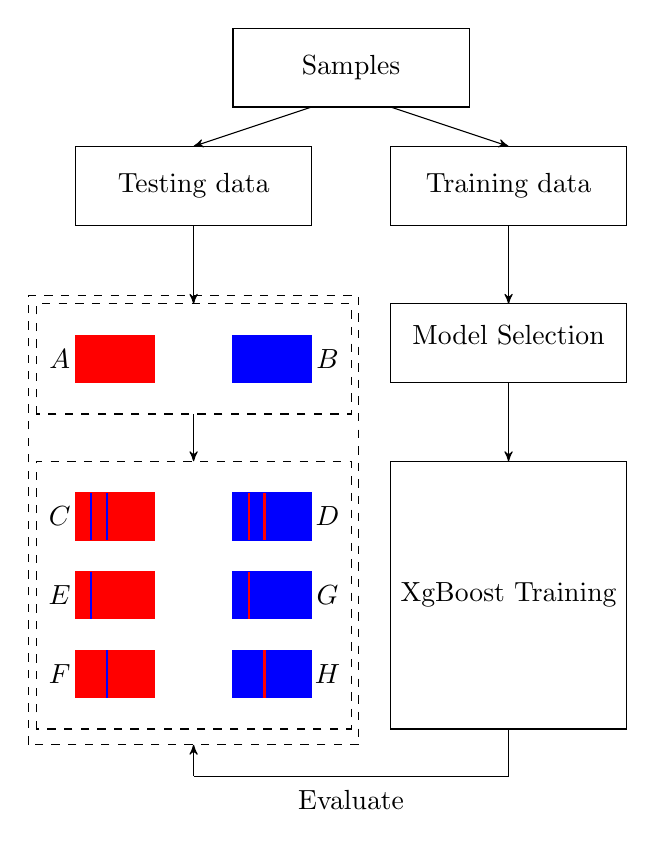
\begin{tikzpicture}
\draw [fill=red,red] (0,5) rectangle (1,5.6);
\draw [fill=red,red] (0,3) rectangle (1,3.6);
\draw [fill=red,red] (0,2) rectangle (1,2.6);
\draw [fill=red,red] (0,1) rectangle (1,1.6);
\draw [fill=blue,blue] (2,5) rectangle (3,5.6);
\draw [fill=blue,blue] (2,3) rectangle (3,3.6);
\draw [fill=blue,blue] (2,2) rectangle (3,2.6);
\draw [fill=blue,blue] (2,1) rectangle (3,1.6); 
\node at (-0.2,5.3){$A$};
\node at (-0.2,3.3){$C$};
\node at (-0.2,2.3){$E$};
\node at (-0.2,1.3){$F$};
\node at (3.2,5.3){$B$};
\node at (3.2,3.3){$D$};
\node at (3.2,2.3){$G$};
\node at (3.2,1.3){$H$};
\draw[thick,blue](0.2,3.6)--(0.2,3);
\draw[thick,blue](0.4,3.6)--(0.4,3);
\draw[thick,blue](0.2,2.6)--(0.2,2);
\draw[thick,blue](0.4,1.6)--(0.4,1);
\draw[thick,red](2.2,3.6)--(2.2,3);
\draw[thick,red](2.4,3.6)--(2.4,3);
\draw[thick,red](2.2,2.6)--(2.2,2);
\draw[thick,red](2.4,1.6)--(2.4,1);
\draw[dashed] (-0.5,0.6) rectangle (3.5, 4);
\draw[dashed](-0.5,4.6) rectangle (3.5, 6);
\draw[dashed](-0.6,0.4)rectangle(3.6,6.1);
\draw[->](1.5,4.6)--(1.5,4);
\draw[-] (0,7) rectangle (3,8);
\node at (1.5,7.5) {Testing data};
\draw[->](1.5,7)--(1.5,6);
\draw[-] (4,7) rectangle (7,8);
\node at (5.5,7.5) {Training data};
\draw[-] (4,0.6) rectangle (7,4);
\draw[-] (4,5) rectangle (7,6);
\node at (5.5, 5.6) {Model Selection};
\draw[->](5.5,5)--(5.5,4);
\node at (5.5, 2.3) {XgBoost Training};
\draw[->] (5.5,7)--(5.5,6);
\draw[-] (2, 8.5)rectangle (5,9.5);
\node at (3.5,9) {Samples};
\draw[->](3,8.5)--(1.5,8);
\draw[->](4,8.5)--(5.5,8);
\draw[-](5.5,0.6)--(5.5,0)--(1.5,0);
\draw[->](1.5,0)--(1.5,0.4);
\node at (3.5,-0.3) {Evaluate};
\end{tikzpicture}
    \end{center}
\caption{\label{fig1} The framework of gpXGB}
\end{figure}

Hence, the learning objective is
\begin{equation}
obj=\sum_i(l(y_i,\hat{y}(x_i))+\sum_k\Omega(f_k)
\end{equation}
Where $l(y,\hat{y})=y\log(1+e^{-\hat{y}})+(1-y)\log(1+e^{\hat{y}})$ is the logistic regression loss function, and $\Omega(f_k)$ is the regularizer.

\paragraph{Gradient Boosting}
It is not feasible to train all the trees in the ensemble together at once because it is hard to calculate the gradient as which is needed in traditional optimization methods. Instead, Xgboost use an additive training strategy: fix the trees have already learned, add new trees one at a time. Let $\hat{y}^{(t)}$ be the
predictor at iteration $t$, then
\begin{equation}
\hat{y}^{(0)}=0
\end{equation}
\begin{equation}
\hat{y}^{(t)}=\hat{y}^{(t-1)}+f_t
\end{equation}
Where $f_t\in\mathcal{F}$ optimizes the following target function, which is obtained by the Taylor expansion of the lost function for logistic regression to the second order.
\begin{equation}
obj^t=\sum_i\left(g_i(\hat{y}^{(t-1)}(x_i))f_t(x_i)+{h_i^2(\hat{y}^{(t-1)}(x_i))\over 2}\cdot f_t^2(x_i)\right)+\Omega(f_i)
\end{equation}
Here $g_i(\hat{y})={d\over d\hat{y}}l(y_i,\hat{y})$, $h_i(\hat{y})={d\over d\hat{y}}l(y_i,\hat{y})$.

\paragraph{Regularizer and Training strategy for CARTs}

For any $f\in\mathcal{F}$ , let $T$ be the number of leaves in the tree representing $f$ , $w_1,\dots, w_T$ be the scores on
the leaves. Then the regularizer used in XGBoost is
\begin{equation}
\Omega(f)=\gamma T+{1\over 2}\lambda\sum_j w_j^2
\end{equation}
The purpose of the second term is that it can smoothen the leaf scores.

To optimize $f_t$, firstly note that given a tree structure, $obj^t$ is a quadratic function of the scores $w_j$,
and the minimum of $obj^t$ as well as the $w_j$ that minimizes $obj^t$ can be easily calculated given the tree structure. Now the tree can be constructed by a greedy algorithm in which one starts with a tree with
one single node, and repeatedly split its leaves in a way that maximizes the decrease in $obj^t$ in each step.

% \subsubsection{Permutation}

% The idea of detecting SNP interaction through permutation has previously been used by Greene \cite{10}
% and Jing \cite{2}.Greene et al. designed an explicit test of epistasis to reflect only nonlinear interaction
% or epistasis component of the model. They advanced the traditional permutation testing framework
% by shuffling each SNP column instead of randomizing the class label, which can generate permuted
% datasets for testing the null hypothesis that the only genetic associations in the data are linear or
% additive in nature and that any nonlinear interaction effects are only there by chance. This yields an
% explicit test of epistasis when combining with a method such as MDR, is capable of modeling
% nonlinear interactions. Jing et al. developed a permuted Random Forest (pRF) method. They
% generated two test dataset by permutating the genotype of a pair of SNPs. In one dataset the SNPs
% are shuffled independently, while in the other they are shuffled as a pair hence keeping the pairwise
% association. The difference of error rate between the two test dataset on a well-trained RF model is
% then used to measure the strength of the interaction of selected SNP pair. Other SNPs except for the
% selected pair kept their original form in both dataset, so the interactions among other non-selected
% SNPs were preserved in both of the permutation framework.\\

% Both methods above are marker-based. Motivated by them, we designed a gene-based permutation
% strategy for our interaction detection. For each pair of genes, we carried out two permutation
% strategies to generate two test datasets. Firstly, we divide the samples by class label into case and
% control groups. Then, in the first permutation strategy, we shuffle the genotype of all the genes
% independently among the samples within each group, which removes all associations between geneswithin each group while keeping the association between SNPs within each gene. The independent
% margin effect of each gene is preserved due to the unchanged genotype frequencies of each gene
% within each group before and after permutation. In the second permutation strategy, within both the
% case and the control group, the genotypes of the two chosen genes are shuffled together as a group
% while the genotypes of all other genes are shuffled independently. Hence, the difference between
% the two test dataset is merely the presentation or deletion of the interaction between the pair of genes.\\

% Comparing with the approach of Jing etc., our approach is gene-based as opposed to marker-based,
% hence is more suitable for detecting interaction between genes. Also, in selecting interaction terms
% we used a forward selection strategy instead of the backward selection strategy used by Jing etc.
% (emphasize the difference between our permutation and Jing’s)

\subsubsection{Testing and Ranking}

Our approach for gene-based gene-gene interaction detection is based testing the extend a model trained with XGBoost (c.f. section 2.2) deviate from the ``product form'' in Equation (1). Our interaction estimation
technique is based on the following observation: if Equation (1) is satisfied for $g, g'$, and let $\mathcal{P}(X_1,\dots, X_G):=P(y=1|X_1,\dots, X_G)$, $X_0$ be the vector consisting of features that are in neither $X_g$ nor $X_{g'}$, then, for any two genotypes $(X_k)$, $(X'_k)$, we have
\begin{equation*}
\mathcal{P}(X_g, X_{g'}, X_0)\mathcal{P}(X'_g,X'_{g'},X'_0)\mathcal{P}(X'_g,X'_{g'},X_0)\mathcal{P}(X_g,X_{g'},X'_0)
\end{equation*}
\begin{equation}=\mathcal{P}(X'_g,X_{g'},X_0)\mathcal{P}(X_g,X'_{g'},X'_0)\mathcal{P}(X'_g,X_{g'},X'_0)\mathcal{P}(X_g,X'_{g'},X_0)
\end{equation}
To verify that, note that if $\mathcal{P}(X_g, X_{g'}, X_0)=F_g(X_g, X_0)F_{g'}(X_{g'},X_0)$, then the left-hand-side of equation (8) above becomes:
$F_g(X_g,X_0)F_{g'}(X_{g'},X_0)F_g(X'_g,X'_0)F_{g'}(X'_{g'},X'_0)F_g(X'_g,X_0)\\F_{g'}(X'_{g'},X_0)F_g(X_g,X'_0)F_{g'}(X_{g'},X'_0)$, 
while the right-hand-side becomes:
$F_g(X'_g,X_0)F_{g'}(X_{g'},X_0)\\F_g(X_g,X'_0)F_{g'}(X'_{g'},X'_0)F_g(X'_g,X'_0)F_{g'}(X_{g'},X'_0)F_g(X_g,X_0)F_{g'}(X'_{g'},X_0)$.
It is evident that these two are the same.\\

This observation is motivated by the well-known fact that a function $f(X,Y)$ is of the form $f(X,Y)=u(X)v(Y)$ if and only if for any $a,b,c,d$, $f(a,b)f(c,d)=f(a,d)f(c,b)$.\\

As the function $\mathcal{P}$ is unknown, we use the predicted probability of XgBoost as an estimator of it. We test equation (8) on a testing set drawn from the same original sample set as the training set we used to train XgBoost model, because we want the distribution of the genotypes tested to be closer to the distribution of the genotype of the training data in order to minimize the error caused by interpolation.\\

With the considerations above, we propose our ranking algorithm as follows: 

\begin{algorithm}[H]
\SetAlgoLined
\SetKwInOut{Input}{input}
\SetKwInOut{Output}{output}
\Input{genotype dataset $S=\{(x_1,y_1),(x_2,y_2)\dots (x_n,y_n)\}, x_i\in \mathbb\{0,1,2\}^{(m_1,\dots m_G)}, y_i\in \{0,1\} $; gene list file with position information for the $G$ genes; buffer region size.}
\Output{A list of all pairs of genes sorted by $\Delta AUC$.}
Train Xgboost model, using grid search to find the proper parameter combination of the Xgboost, using 5-fold cross validation for each parameter combination and select the best parameter combination that gives the best average predictive performance.\\
\For{$i=1,\dots N$}{
Divide dataset $S$ randomly into a training and a testing set.\\
XgboostModel = trainXgboost($S$, parameter combination)\\
Sample the testing dataset to obtain two sets of genotype data $A=\{{X^A}^i\}$ and $B=\{{X^B}^i\}$ of equal size.\\
\For{$1\leq g<g'\leq G$}{
Let $C=\{{X^C}^i\}$ be a set of genotypes, which has the same genotype as $A$ on all genes except the $g$ and the $g'$-th, and the same genotype as $B$ on the $g$ and the $g'$-th.\\
Let  $D=\{{X^D}^i\}$ be a set of genotypes, which has the same genotype as $B$ on all genes except the $g$ and the $g'$-th, and the same genotype as $A$ on the $g$ and the $g'$-th.\\
Let  $E=\{{X^E}^i\}$ be a set of genotypes, which has the same genotype as $A$ on all genes except the $g$-th, and the same genotype as $B$ on the $g$-th.\\
Let  $F=\{{X^F}^i\}$ be a set of genotypes, which has the same genotype as $A$ on all genes except the $g'$-th, and the same genotype as $B$ on the $g'$-th.\\
Let  $G=\{{X^G}^i\}$ be a set of genotypes, which has the same genotype as $B$ on all genes except the $g$-th, and the same genotype as $A$ on the $g$-th.\\
Let  $H=\{{X^H}^i\}$ be a set of genotypes, which has the same genotype as $B$ on all genes except the $g'$-th, and the same genotype as $A$ on the $g'$-th.
$\Delta P_{g,g'}=\sum_i(Predict(XgBoostModel, {X^A}^i)Predict(XgBoostModel, {X^B}^i)$\\
$Predict(XgBoostModel, {X^C}^i)Predict(XgBoostModel, {X^D}^i)-$\\
$Predict(XgBoostModel, {X^E}^i)Predict(XgBoostModel, {X^F}^i)$\\
$Predict(XgBoostModel, {X^G}^i)Predict(XgBoostModel, {X^H}^i))$
}
}
Return $C^2_G$ pairs of genes sorted by the total $\Delta P_{g,g'}$ in all $N$-iterations in decreasing order.
 \caption{gpXGB}
\end{algorithm}

% \subsubsection{Interpretation of the algorithm}

% Let $F(X_1,X_2)=P(y=1|X_1,X_2)$, and suppose the machine learning algorithm can capture $F$ perfectly. Then, the expected ROC after the permutation of the second type is
% \begin{equation}
% \left(\sum_{F(a,b)>p}P(X_1=a,X_2=b|Y=0),1-\sum_{F(a,b)<p}P(X_1=a,X_2=b|Y=1)\right)
% \end{equation}
% while the expected ROC of the permutation of the first type is:
% \begin{equation}
% \left(\sum_{F(a,b)>p}P(X_1=a|Y=0)P(X_2=b|Y=0),1-\sum_{F(a,b)<p}P(X_1=a|Y=1)P(X_2=b|Y=1)\right)
% \end{equation}

% Hence, the expected $\Delta AUC$ is
% \begin{align*}
% &\int_0^1\left(1-\sum_{F(a,b)<p}P(X_1=a,X_2=b|Y=1)\right)\\
% & d\left(\sum_{F(a,b)>p}P(X_1=a,X_2=b|Y=0)\right)-\\
% &\int_0^1 \left(1-\sum_{F(a,b)<p}P(X_1=a|Y=1)P(X_2=b|Y=1)\right)\\
% & d\left(\sum_{F(a,b)>p}P(X_1=a|Y=0)P(X_2=b|Y=0)\right)
% \end{align*}

% In particular, the AUCs are the same if $X_1$ and $X_2$ are conditionally independent with regards to $Y$.


\subsection{Simulation study}

The goal of this simulation study is to evaluate the performance of gpXGB procedure for gene-gene interaction detection. All simulated datasets were set to have 50 SNPs. Among them 2 SNPs were functional and the remaining 48 SNPs were non-functional. The 50 SNPs formed 5 genes, each had 10 SNPs. The 2 functional SNPs were put into the first and second gene, and the performance is measured by how likely our algorithm can rank the two interacting genes as the most significant. We chose the publicly available tool GAMETES \cite{11} to generate the simulated genotype data. This tool is designed to generate epistasis models that we refer to as pure and strict. Purely and strictly epistasis models constitute the most difficult type of disease association model to detect, as such associations may be observed only if all n-loci are included in the disease model. This requirement makes these types of models an attractive gold standard for simulation studies of complex multi-locus effects. \\

In this simulation study, to test the effects of heritability (which measures the strength of correlation between genotype and phenotype) and sample size, we performed experiments under two different scenarios. In the first scenario, we tested two locus epistasis models with five different heritability (0.01, 0.025, 0.05, 0.1 and 0.2) and two different minor allele frequencies (0.2 and 0.4) with prevalence set to be 0.2 and sample size to be 3000. Ten models for each of the 10 heritability-allele frequency combinations were generated, so that we had 100 models in total in accordance to Hardy-Weinberg proportions. The penetrance tables were generated for these 100 models in the absence of main effect. One hundred datasets were generated from each model with balanced cases and controls,resulting in 10000 datasets in total in this scenario. In the second scenario, we set heritability to be (XX, XX) and MAF to be 0.2, prevalence to be XX with sample size 10000. Then, 100 datasets were generated by random sampling from this large dataset for each of the 5 sample sizes 1000, 2000, 3000, 4000 and 5000. In this scenario, we have 500 datasets in total.\\

\subsection{Real data analysis}
To assess the capacity of gpXGB to deal with real case-control phenotype, we first investigated the susceptibility of a set of pairs of genes to Rheumatoid Arthritis (RA), a chronic autoimmune joint disease where persistent inflammation affects bone remodeling leading to progressive bone destruction. We used the GSE39428 dataset for which genotyping is performed using a custom-designed Illumina 382-SNP VeraCode microarray (Illumina, San Diego, CA, USA) to determine possible associations of genes to RA. The dataset contains 266 cases and 163 controls. After preprocessing, we obtain 381 SNPs encoding 17 genes. Next, we used the WTCCC dataset as a replication cohort WTCCC (2007). The datasets were genotyped in the British population using the Affymetrix GeneChip 500k. Quality control was performed in PLINK with several steps. First we removed samples with reported sex that did not 
match the heterozygosity rates observed on chromosome X \cite{12}. We additionally filtered out SNPs with $>10\%$ missingness,  with a minor allele frequency (MAF) $<0.05$, or for which missingness was significantly correlated with 
phenotype ($p<1\times 10^{-4}$). We further filter out SNPs that are not in Hardy-Weinberg equilibrium in controls, as well as filter out samples with $>10\%$ missing SNPs. After the QC steps, we have XX SNPs, XXX samples with XXX cases and XXX controls.\\

In a second analysis, we aim to verify some gene-gene interaction in the RA pathway hsa05323 in KEGG pathway dataset. Genotyping coordinates are given in NCBI Build36/UCSC hg18 (National Center for Biotechnology Information, Bethesda, MD). There are XX genes in the pathway, and we can mapping XX based on Build36 annotation. For each gene, we add 10k to both the upstream and downstream. Gender was included as covariate in the analysis. Principal component analysis was conducted using GCAT[], and top 10 PCs were also included as covariates to account for potential population stratification.\\

\subsection{Competitive methods}
The performance of our procedure gpXGB was compared to three previously published methods: Kernel Canonical Correlation-based U-statistic analysis (KCCU)\cite{4, 5}, the gene-based information gain method (GBIGM)\cite{6} and A Gene-based Gene-Gene interaction test method (AGGrEGATOr)\cite{7}. We adapted them to the task of ranking, by ranking the gene pairs by their p-values in ascending order.

\section{Results}

\subsection{Results for the simulation study}

Figure~\ref{det} shows the performance of gpXGB and various other approaches on the simulated datasets with different heritability. Figure~\ref{avg} shows the relationship between heritability and the average performance. Here, the number for ``gpXGB'' is the relative frequency for gpXGB to rank the single interacting gene pair as the first, and ``gpXGB\_under 0.01'' is the relative frequency for two runs of the gpXGB both ranking the single interacting gene pair as the first. For all other methods, the number listed is the relative frequency for the single interacting pair to have the smallest p-value.

\begin{figure}[H]
    \begin{center}
       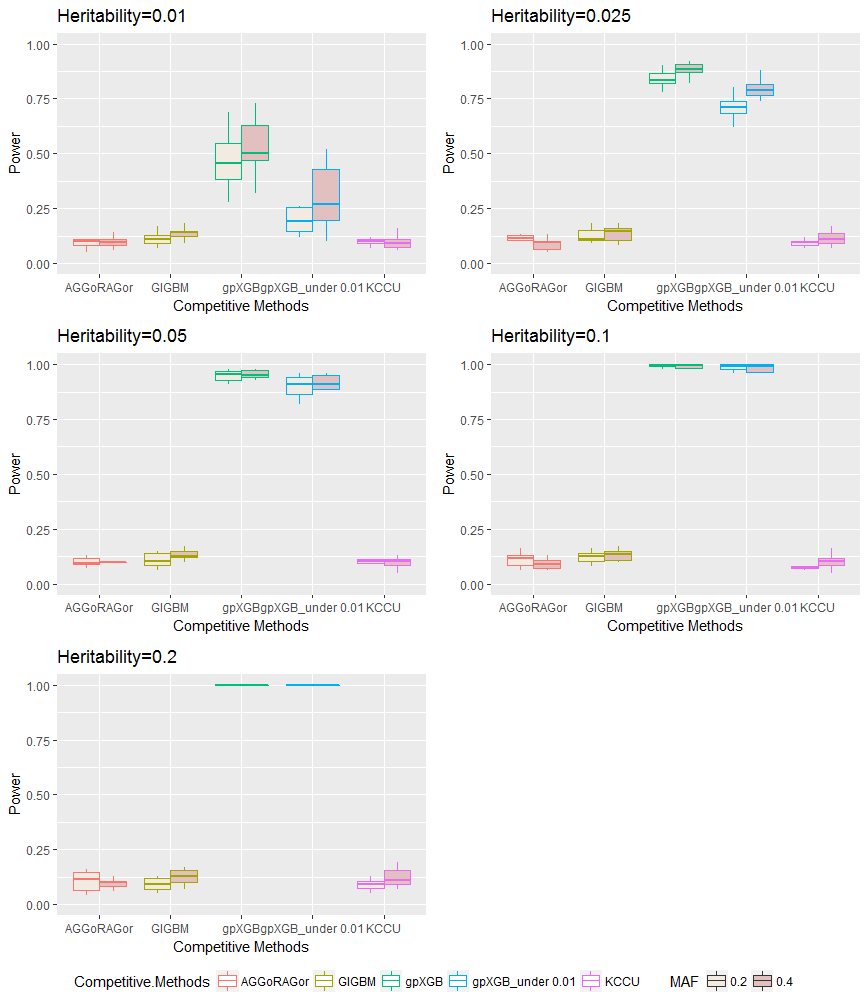
\includegraphics[scale=0.6]{Rplot02.png}
    \end{center}
\caption{\label{det}Performance on the simulated datasets}
\end{figure}

\begin{figure}[H]
    \begin{center}
       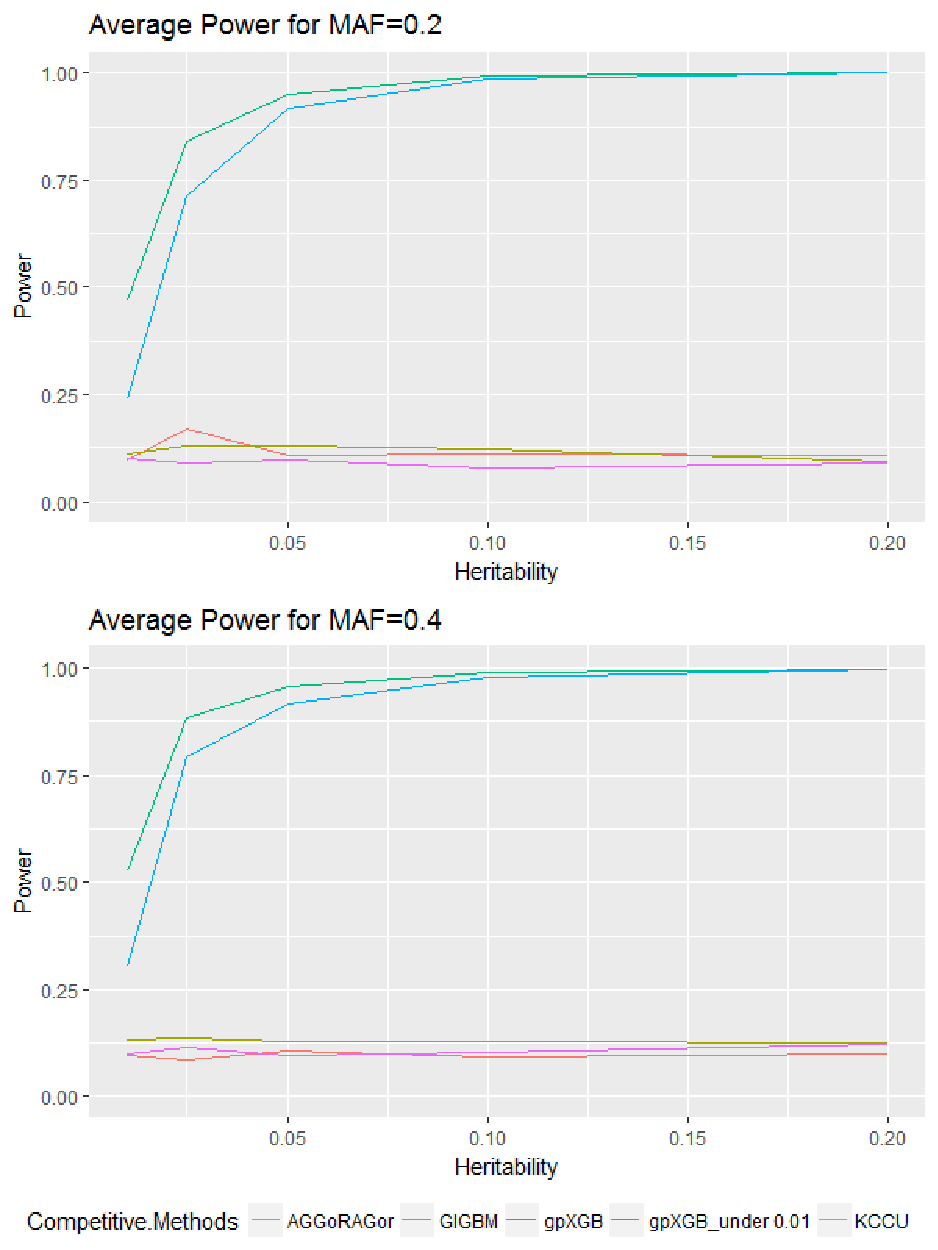
\includegraphics[scale=0.5]{Rplot01}
    \end{center}
\caption{\label{avg}Average performance on the simulated datasets}
\end{figure}

As can be seen in Figure~\ref{avg}, the performance of $gpXGB$ increases with the heritability.


\section{Discussion}

In this paper, we proposed a new machine learning algorithm based procedure, called gpXGB, to detect interaction at the gene level by applying the XGBoost and permutation strategies. We proved the capacity of gpXGB to detect gene interaction, especially for the pure and strict type interactions. According to a power study based on a wide range of disease models with different combination with heritability and MAF, gpXGB is shown to be the most powerful method when one causal pair is associated with the case-control phenotypes.\\

In the gpXGB procedure, we consider the interaction between two genes as an additive model, each additive term represent some kind of non-linear interaction between SNPs from the two genes. We did not model the interactions form between SNPs explicity. Such assumption made the method more powerful compared to AGGrEGATOr or KCCU. Our Method also can include the covariates matrix, which can correct confounding information such as population stratification with no more computational resources. Necessary for GWAS. We have applied a version with parallelize calculation for the permutation.\\

The application of gpXGB procedure to the association between RA and 43 genes from RA pathway confirmed that the capacity for gpXGB to be a robust and valid method compared to competitive methods and also gives promising new insights in the etiology of RA.\\

Genome-wide implementation of gpXGB is hardly feasible since the input of the model is all the candidate genes, too many unrelated genes may be harmful for the performance of the XGBoost model. To avoid the computational all the gene pairs, another strategy consists in using prior biological knowledge to reduce the number of genes need to be considered. Indeed, gpXGB procedure can easily be used in a network –based approach since it is widely assumed that protein-protein interaction network or pathway-based approach can be successfully combined to GWAS. Furthermore, the term “gene” refers to a collection of SNPs and can be any locus, even some non-function unit such as non-coding RNA. For all the reason we believe that the gpXGB procedure can help detecting part of the missing heritability.


\section{Conflict of interest}

\section{Acknowledgements}

\begin{thebibliography}{9}
\bibitem{1}Wan, X., et al., {\em BOOST: A fast approach to detecting gene-gene interactions in genome-wide case-control studies}. Am J Hum Genet, 2010. 87(3): p. 325-40.
\bibitem{2}Li, J., et al., {\em Detecting gene-gene interactions using a permutation-based random forest method}. BioData Min, 2016. 9: p. 14.
\bibitem{3}Peng, Q., J. Zhao, and F. Xue, {\em A gene-based method for detecting gene-gene co-association in a case-control association study}. Eur J Hum Genet, 2010. 18(5): p. 582-7.
\bibitem{4}Yuan, Z., et al., {\em Detection for gene-gene co-association via kernel canonical correlation analysis}. BMC Genet, 2012. 13: p. 83.
\bibitem{5}Larson, N.B., et al., {\em Kernel canonical correlation analysis for assessing gene-gene interactions and application to ovarian cancer}. Eur J Hum Genet, 2014. 22(1): p. 126-31.
\bibitem{6}Li, J., et al., {\em A gene-based information gain method for detecting gene-gene interactions in case-control studies}. Eur J Hum Genet, 2015. 23(11): p. 1566-72.
\bibitem{7}Emily, M., {\em AGGrEGATOr: A Gene-based GEne-Gene interActTiOn test for case-control association studies}. Stat Appl Genet Mol Biol, 2016. 15(2): p. 151-71.
\bibitem{8}Ma, L., A.G. Clark, and A. Keinan, {\em Gene-based testing of interactions in association studies of quantitative traits}. PLoS Genet, 2013. 9(2): p. e1003321.
\bibitem{9}Chen, T. and C. Guestrin. {\em XGBoost: A Scalable Tree Boosting System. in ACM SIGKDD International Conference on Knowledge Discovery and Data Mining}. 2016.
\bibitem{13}Mentch, Lucas, and Giles Hooker, {\em Formal hypothesis tests for additive structure in random forests}. Journal of Computational and Graphical Statistics, 2016.
\bibitem{10}Greene, C.S., et al., {\em Enabling personal genomics with an explicit test of epistasis}. Pac Symp Biocomput, 2010: p. 327-36.
\bibitem{11}Urbanowicz, R.J., et al., {\em GAMETES: a fast, direct algorithm for generating pure, strict, epistatic models with random architectures}. BioData Min, 2012. 5(1): p. 16.
\bibitem{12}Laurie, C.C., et al., {\em Quality control and quality assurance in genotypic data for genome-wide association studies}. Genet Epidemiol, 2010. 34(6): p. 591-602.



\end{thebibliography}



\end{document}
